% ============================================================
%  RELATÓRIO — ARQUITETURAS DE ALTO DESEMPENHO
%  Prática 7: Arquitetura Mesh 4×4 para PDI com Roteamento XY
%  Normas para Elaboração de Relatórios ver 4 (2026)
%  Universidade Federal de São Carlos (UFSCar)
% ============================================================
\documentclass[12pt, a4paper]{article}

% --- Codificação e idioma ---
\usepackage[utf8]{inputenc}
\usepackage[T1]{fontenc}
\usepackage[brazil]{babel}
\usepackage{amsmath}
\usepackage{amssymb}
\usepackage{multirow}

% --- Fonte Times New Roman ---
\usepackage{mathptmx}

% --- Geometria da página ---
\usepackage[
top=2.5cm,
bottom=2.5cm,
left=3.0cm,
right=3.0cm
]{geometry}

% --- Espaçamento entre linhas ---
\usepackage{setspace}
\onehalfspacing

% --- Indentação do parágrafo ---
\usepackage{indentfirst}
\setlength{\parindent}{1.25cm}

% --- Pacotes gráficos e de figuras ---
\usepackage{graphicx}
\usepackage{float}

% --- Tabelas ---
\usepackage{booktabs}
\usepackage{array}
\usepackage{longtable}

% --- Listagens de código ---
\usepackage{listings}
\usepackage{xcolor}

\lstdefinestyle{verilog}{
	language=Verilog,
	basicstyle=\ttfamily\small,
	keywordstyle=\color{blue}\bfseries,
	commentstyle=\color{gray}\itshape,
	stringstyle=\color{teal},
	numbers=left,
	numberstyle=\tiny\color{gray},
	stepnumber=1,
	numbersep=8pt,
	frame=single,
	breaklines=true,
	breakatwhitespace=true,
	columns=flexible,
	keepspaces=true,
	captionpos=b,
	morekeywords={module,endmodule,input,output,reg,wire,always,begin,end,
		posedge,negedge,if,else,case,endcase,assign,parameter,
		localparam,integer,initial,for,while,task,endtask,defparam}
}

\lstdefinestyle{vhdl}{
	language=VHDL,
	basicstyle=\ttfamily\small,
	keywordstyle=\color{blue}\bfseries,
	commentstyle=\color{gray}\itshape,
	stringstyle=\color{teal},
	numbers=left,
	numberstyle=\tiny\color{gray},
	stepnumber=1,
	numbersep=8pt,
	frame=single,
	breaklines=true,
	breakatwhitespace=true,
	columns=flexible,
	keepspaces=true,
	captionpos=b,
}

% --- Numeração de seções ---
\setcounter{secnumdepth}{3}

% --- Cabeçalho e rodapé ---
\usepackage{fancyhdr}
\setlength{\headheight}{14pt}
\pagestyle{fancy}
\fancyhf{}
\fancyhead[R]{\small Arquiteturas de Alto Desempenho --- Relatório}
\fancyfoot[C]{\thepage}
\renewcommand{\headrulewidth}{0.4pt}

% --- Hiperlinks (DEVE ser o último pacote) ---
\usepackage[hidelinks]{hyperref}

% ============================================================
%  INÍCIO DO DOCUMENTO
% ============================================================
\begin{document}
	
	\thispagestyle{empty}
	
	% ============================================================
	%  CAPA
	% ============================================================
	\begin{titlepage}
		\centering
		
		\noindent\rule{\textwidth}{0.8pt}\\[0.2cm]
		{\large \textbf{UNIVERSIDADE FEDERAL DE SÃO CARLOS}}\\[0.15cm]
		{\normalsize Centro de Ciências Exatas e Tecnologia}\\[0.15cm]
		{\normalsize Departamento de Computação}\\[0.15cm]
		
		\vspace{0pt plus 0.35fill}
		
		{\large \textbf{Laboratório de Arquiteturas de Alto Desempenho}}\\[0.4cm]
		{\large Prática 7 --- Arquitetura Mesh 4$\times$4 para\\[0.2cm]
			Processamento Digital de Imagens com Roteamento XY}\\[1.0cm]
		{\normalsize Professor: \textit{Dr. Emerson Carlos Pedrino}}\\
		
		\vspace{0pt plus 0.65fill}
		
		\begin{center}
			{\normalsize \textit{Pedro Augusto Faria} \ (RA: \textit{821124})}\\[0.15cm]
			{\normalsize Curso: \textit{Engenharia da Computação}}\\[0.15cm]
		\end{center}
		
	\end{titlepage}
	
	\setcounter{page}{1}
	
	% ============================================================
	%  SEÇÃO 1 — INTRODUÇÃO
	% ============================================================
	\section{Introdução}
	
	As redes intra-chip (\textit{Network-on-Chip}, NoC) representam um paradigma
	arquitetural fundamental para sistemas de processamento paralelo de alto
	desempenho implementados em hardware reconfigurável. Em substituição aos
	barramentos compartilhados tradicionais, as NoCs oferecem comunicação
	escalável, de alta largura de banda e baixa latência entre múltiplos núcleos
	de processamento (\textit{Processing Elements}, PEs) dispostos em topologias
	regulares --- sendo a malha bidimensional (\textit{mesh}) a mais empregada
	na literatura e na indústria.
	
	Nesta prática, implementa-se uma rede \textit{mesh} 4$\times$4 em FPGA para
	o processamento digital de imagens (PDI), especificamente para a aplicação do
	filtro \textit{sal e pimenta} (filtro de máximo e mínimo sobre janela de
	$3\times3$ pixels). A rede é composta por 16 nós (\texttt{mesh\_node}), cada
	um dotado de um núcleo de processamento (\texttt{modulo\_sal\_e\_pimenta}) e
	de um roteador com política de roteamento determinístico XY. Os dados de
	imagem provenientes de uma ROM são injetados no nó de entrada, roteados pela
	rede conforme um caminho configurável de até quatro saltos (\textit{hops}), e
	a saída do nó final é exibida em monitor VGA de resolução 640$\times$480.
	
	O roteamento XY (\textit{dimension-order routing}) garante ausência de
	\textit{deadlock} na rede ao impor que o pacote se desloca primeiro na direção
	horizontal (eixo $x$, colunas) até alinhar-se com a coluna destino, e somente
	então na direção vertical (eixo $y$, linhas). Esta política é implementada
	localmente em cada nó, sem necessidade de tabelas de roteamento globais,
	tornando-a escalável e sintetizável de forma compacta em FPGA.
	
	O módulo controlador \texttt{noc\_controller} define estaticamente os
	endereços e os modos de operação (máximo ou mínimo) dos quatro nós do caminho
	de processamento ativo, permitindo a experimentação rápida de diferentes
	configurações de roteamento --- coluna vertical, grupo no topo, ou diagonal
	--- simplesmente alternando atribuições de constantes no código.
	
	\subsection{Fundamentação Teórica}
	
	\subsubsection{Redes \textit{Mesh} e Roteamento XY}
	
	Uma rede \textit{mesh} $M \times N$ é um grafo regular em que cada nó
	$(col, row)$ está conectado a até quatro vizinhos: norte $(col, row-1)$,
	sul $(col, row+1)$, leste $(col+1, row)$ e oeste $(col-1, row)$. Os nós das
	bordas possuem menos conexões (sem vizinho externo). A topologia é atraente
	por sua regularidade, que facilita o roteamento e o leiaute físico.
	
	O roteamento XY é um algoritmo de roteamento determinístico e livre de
	\textit{deadlock} para redes \textit{mesh} bidimensionais. Dado um nó fonte
	$(c_s, r_s)$ e um nó destino $(c_d, r_d)$, o caminho percorrido é:
	
	\begin{enumerate}
		\item Mover na direção horizontal (leste se $c_d > c_s$, oeste se
		$c_d < c_s$) até que $c_{atual} = c_d$;
		\item Mover na direção vertical (sul se $r_d > r_s$, norte se
		$r_d < r_s$) até que $r_{atual} = r_d$.
	\end{enumerate}
	
	Este ordenamento garante que não há ciclos no grafo de dependência de canais,
	o que é condição suficiente para ausência de \textit{deadlock} \cite{dally}.
	
	\subsubsection{Endereçamento dos Nós}
	
	Na implementação adotada, cada nó é identificado por um endereço de 4 bits
	$\langle col[1:0], row[1:0] \rangle$, onde os dois bits mais significativos
	representam a coluna e os dois menos significativos representam a linha (ambos
	indexados de 0 a 3). Assim, o nó na coluna 1, linha 2 tem endereço
	\texttt{4'b0110}. A Tabela~\ref{tab:enderecos} lista o mapeamento completo
	para a \textit{mesh} 4$\times$4.
	
	\begin{table}[H]
		\centering
		\caption{Mapeamento de endereços para a \textit{mesh} 4$\times$4.}
		\label{tab:enderecos}
		\begin{tabular}{ccccc}
			\toprule
			& \textbf{Col 0} & \textbf{Col 1} & \textbf{Col 2} & \textbf{Col 3} \\
			\midrule
			\textbf{Lin 0} & \texttt{0000} & \texttt{0100} & \texttt{1000} & \texttt{1100} \\
			\textbf{Lin 1} & \texttt{0001} & \texttt{0101} & \texttt{1001} & \texttt{1101} \\
			\textbf{Lin 2} & \texttt{0010} & \texttt{0110} & \texttt{1010} & \texttt{1110} \\
			\textbf{Lin 3} & \texttt{0011} & \texttt{0111} & \texttt{1011} & \texttt{1111} \\
			\bottomrule
		\end{tabular}
	\end{table}
	
	\subsubsection{Filtro Sal e Pimenta}
	
	O filtro \textit{sal e pimenta} é um filtro de ordem estatística utilizado
	para a remoção de ruído impulsivo em imagens digitais. Para cada pixel
	$(x, y)$, considera-se a janela de vizinhança $3\times3$ centrada em $(x,y)$,
	composta por 9 pixels. O filtro de máximo substitui o pixel central pelo
	valor máximo da janela (produz o efeito \textit{sal}), enquanto o filtro de
	mínimo substitui pelo valor mínimo (produz o efeito \textit{pimenta}). Para
	imagens binárias de 1 bit por pixel, os filtros de máximo e mínimo equivalem,
	respectivamente, à dilatação e erosão morfológicas.
	
	Na implementação em hardware, a janela $3\times3$ é construída por meio de
	registradores de deslocamento que modelam linhas de atraso (\textit{line
		buffers}), armazenando os pixels das duas linhas anteriores à linha corrente.
	Dado que a imagem tem largura de 256 pixels (conforme a máscara de janela),
	cada linha de atraso requer 256 registradores de 1 bit.
	
	\subsubsection{Concatenador de Endereços para ROM}
	
	O módulo \texttt{concatenador} (VHDL) forma o endereço de 15 bits para
	acesso à ROM de imagem a partir das coordenadas de pixel do controlador VGA.
	Os 7 bits menos significativos da linha (\texttt{pixel\_row[6:0]}) são
	concatenados com os 8 bits menos significativos da coluna
	(\texttt{pixel\_column[7:0]}), formando um endereço que cobre uma imagem de
	$128 \times 256 = 32.768$ pixels --- correspondente à região de interesse
	definida pela máscara de janela.
	
	\subsubsection{Máscara de Janela}
	
	O módulo \texttt{mascara\_janela} (VHDL) delimita a região ativa de
	processamento da imagem no quadro VGA: apenas pixels com
	\texttt{pixel\_column} $< 256$ e \texttt{pixel\_row} $< 128$ recebem o sinal
	\texttt{video\_out = '1'}. Fora desta região, \texttt{video\_out = '0'}.
	Este sinal de máscara é utilizado em múltiplos pontos do \textit{top-level}
	para habilitar seletivamente o clock da rede \textit{mesh} e a exibição VGA,
	garantindo que o processamento ocorra apenas nos pixels pertencentes à imagem.
	
	\subsection{Objetivos}
	
	\begin{itemize}
		\item Implementar uma rede \textit{mesh} 4$\times$4 em Verilog com
		roteamento determinístico XY na FPGA Altera DE1 (Cyclone II);
		\item Integrar 16 núcleos de processamento \texttt{modulo\_sal\_e\_pimenta}
		como nós da rede, cada um capaz de realizar filtragem de máximo ou mínimo;
		\item Configurar caminhos de processamento de até 4 saltos por meio do
		módulo \texttt{noc\_controller}, experimentando diferentes topologias
		(coluna vertical, grupo no topo, diagonal);
		\item Exibir a imagem original e a imagem filtrada em monitor VGA
		640$\times$480, com seleção de modo por chaves (\textit{switches});
		\item Demonstrar o conceito de NoC aplicada a PDI, evidenciando a
		flexibilidade arquitetural oferecida pelo roteamento XY configurável.
	\end{itemize}
	
	\subsection{Metodologia}
	
	O projeto foi desenvolvido no ambiente Quartus Prime (Versão 24.1std.0 Build
	1077, Lite Edition), com módulos descritos em Verilog e VHDL, integrados por
	diagrama esquemático BDF. O módulo \texttt{VGA\_SYNC} foi fornecido pelo
	professor. Os módulos foram sintetizados para a FPGA Cyclone II EP2C20F484C7
	da placa Altera DE1, com pinagem definida pelo arquivo de pinos oficial.
	
	% ============================================================
	%  SEÇÃO 2 — DESENVOLVIMENTO TEÓRICO
	% ============================================================
	\section{Desenvolvimento Teórico}
	
	\subsection{Topologia da Rede \textit{Mesh} 4$\times$4}
	
	A rede \textit{mesh} 4$\times$4 é composta por 16 nós dispostos em uma grade
	regular de 4 colunas por 4 linhas, totalizando 24 enlaces bidirecionais
	internos (12 horizontais e 12 verticais). Cada nó possui até 4 portas de
	comunicação (norte, sul, leste, oeste), e os nós de borda têm as portas sem
	vizinho conectadas a zero. A Figura~\ref{fig:top_bdf} apresenta o diagrama
	BDF do \textit{top-level}, onde a instância \texttt{mesh\_4x4} concentra toda
	a estrutura da rede.
	
	O fluxo de dados na rede é serial (1 bit por ciclo de clock), compatível com
	a natureza do sinal de vídeo VGA, que também é serial: os pixels chegam em
	sequência, linha por linha, ao longo do quadro. O clock da rede é derivado
	diretamente do pixel clock VGA, habilitado apenas durante a região ativa da
	imagem (controlado pelo sinal \texttt{clk2 = mask \& pclk \& on}), garantindo
	que os registradores de deslocamento internos ao \texttt{modulo\_sal\_e\_pimenta}
	avancem exatamente um pixel por ciclo ativo.
	
	\subsection{Roteamento XY na Implementação}
	
	Na implementação do módulo \texttt{mesh\_node}, o roteamento XY é realizado
	comparando a posição atual do nó (extraída do parâmetro \texttt{MY\_ADDR})
	com a posição do próximo nó no caminho de processamento (\texttt{next\_addr}).
	As quatro decisões de roteamento são lógica combinacional pura:
	
	\begin{align}
		\texttt{go\_s} &= \texttt{on\_path} \wedge \neg\texttt{is\_hop4} \wedge (my\_row < next\_row) \label{eq:go_s}\\
		\texttt{go\_n} &= \texttt{on\_path} \wedge \neg\texttt{is\_hop4} \wedge (my\_row > next\_row) \label{eq:go_n}\\
		\texttt{go\_e} &= \texttt{on\_path} \wedge \neg\texttt{is\_hop4} \wedge (my\_row = next\_row) \wedge (my\_col < next\_col) \label{eq:go_e}\\
		\texttt{go\_w} &= \texttt{on\_path} \wedge \neg\texttt{is\_hop4} \wedge (my\_row = next\_row) \wedge (my\_col > next\_col) \label{eq:go_w}
	\end{align}
	
	Nota-se que a prioridade implícita das condições em \eqref{eq:go_s}--\eqref{eq:go_w}
	implementa o roteamento XY: a comparação de colunas (\texttt{go\_e},
	\texttt{go\_w}) é condicionada à igualdade de linhas (\texttt{my\_row =
		next\_row}), o que significa que o pacote só se desloca horizontalmente
	após ter atingido a linha do destino. Contudo, como nesta implementação o
	deslocamento vertical é processado primeiro (a condição de linha é verificada
	antes da condição de coluna na cadeia de prioridade), a ordem efetiva é
	YX, não XY. Isto não afeta a corretude do roteamento para a topologia
	\textit{mesh} simples, mas é uma nuance de implementação a considerar.
	
	\subsection{Cadeia de Processamento e Seleção de Modo}
	
	O caminho de processamento é definido por quatro endereços de salto
	(\texttt{hop1\_addr} a \texttt{hop4\_addr}) e quatro bits de modo
	(\texttt{hop1\_max} a \texttt{hop4\_max}), todos provenientes do módulo
	\texttt{noc\_controller}. O nó \texttt{hop1} recebe diretamente o dado de
	entrada da ROM (\texttt{din\_entry}); os nós \texttt{hop2}, \texttt{hop3} e
	\texttt{hop4} recebem o dado processado pelo nó anterior via roteamento.
	
	Em cada nó do caminho, o módulo \texttt{modulo\_sal\_e\_pimenta} processa o
	fluxo serial de pixels e produz dois sinais: \texttt{max\_bit} (resultado do
	filtro de máximo) e \texttt{min\_bit} (resultado do filtro de mínimo). O bit
	\texttt{my\_max} seleciona qual dos dois é encaminhado para o próximo nó:
	
	\begin{equation}
		\texttt{pe\_out} = \texttt{my\_max} \;?\; \texttt{pe\_max\_out} : \texttt{pe\_min\_out}
		\label{eq:pe_out}
	\end{equation}
	
	O nó \texttt{hop4} (destino final) disponibiliza \texttt{pe\_out} no sinal
	\texttt{dout\_final}, que é coletado pelo \textit{top-level} e exibido no VGA.
	Os nós fora do caminho simplesmente retransmitem o dado recebido sem processá-lo.
	
	\subsection{Configurações de Roteamento Disponíveis}
	
	O módulo \texttt{noc\_controller} oferece três configurações comentadas no
	código, selecionáveis por descomentação:
	
	\begin{itemize}
		\item \textbf{Coluna vertical} (nós n10 $\to$ n11 $\to$ n12 $\to$ n13):
		percorre a coluna 1 de cima para baixo, com MAX no primeiro e último nó
		e MIN nos intermediários;
		\item \textbf{Grupo no topo} (nós n00 $\to$ n01 $\to$ n11 $\to$ n12):
		forma um L na região superior esquerda da \textit{mesh};
		\item \textbf{Diagonal} (nós n11 $\to$ n12 $\to$ n22 $\to$ n23):
		percorre dois nós verticalmente na coluna 1 e depois dois nós na coluna 2,
		formando uma diagonal na região central da \textit{mesh}. Esta é a
		configuração ativa no código submetido.
	\end{itemize}
	
	\subsection{Sincronismo e Clock Gated}
	
	O uso de \textit{clock gating} (\texttt{clk2 = mask \& pclk \& on}) é uma
	técnica de redução de consumo de energia que desabilita o clock dos
	registradores de deslocamento durante os períodos de \textit{blanking} VGA e
	fora da região de imagem. Em FPGA, o \textit{clock gating} deve ser tratado
	com cuidado para evitar \textit{glitches} no sinal de clock; neste projeto,
	como a lógica de controle (\texttt{mask} e \texttt{on}) é relativamente
	estável durante os períodos críticos, o risco é mitigado.
	
	% ============================================================
	%  SEÇÃO 3 — DESENVOLVIMENTO PRÁTICO
	% ============================================================
	\section{Desenvolvimento Prático}
	\label{sec:pratico}
	
	\subsection{Ambiente de Desenvolvimento}
	
	\begin{table}[H]
		\centering
		\caption{Especificações do ambiente de desenvolvimento.}
		\label{tab:ambiente}
		\begin{tabular}{ll}
			\toprule
			\textbf{Parâmetro}        & \textbf{Valor}                                     \\
			\midrule
			Placa FPGA                & Altera DE1 (Cyclone II EP2C20F484C7)               \\
			Ferramenta EDA            & Quartus Prime 24.1std.0 Build 1077 (Lite Edition)  \\
			Linguagem principal       & Verilog                                            \\
			Linguagem auxiliar        & VHDL (\texttt{concatenador}, \texttt{mascara\_janela}) \\
			Clock da placa            & 50~MHz                                             \\
			Pixel clock VGA           & $\approx$25,175~MHz                                \\
			Resolução VGA             & 640$\times$480 @ 60~Hz                             \\
			Região de imagem ativa    & 256$\times$128 pixels (canto superior esquerdo)   \\
			Topologia da rede         & \textit{Mesh} 4$\times$4 (16 nós)                 \\
			Comprimento do caminho    & 4 saltos configuráveis                             \\
			Filtro implementado       & Sal e pimenta (máximo e mínimo, janela $3\times3$) \\
			Sistema Operacional       & Ubuntu 24.04.4 LTS (Kubuntu)                       \\
			\bottomrule
		\end{tabular}
	\end{table}
	
	\subsection{Estrutura Geral do Projeto e Diagrama de Blocos}
	
	O sistema é integrado pelo módulo \textit{top-level} \texttt{vga\_filtro}
	por meio do editor de esquemáticos BDF do Quartus Prime. A
	Figura~\ref{fig:top_bdf} apresenta o diagrama BDF representativo do sistema
	completo.
	
	\begin{figure}[H]
		\centering
		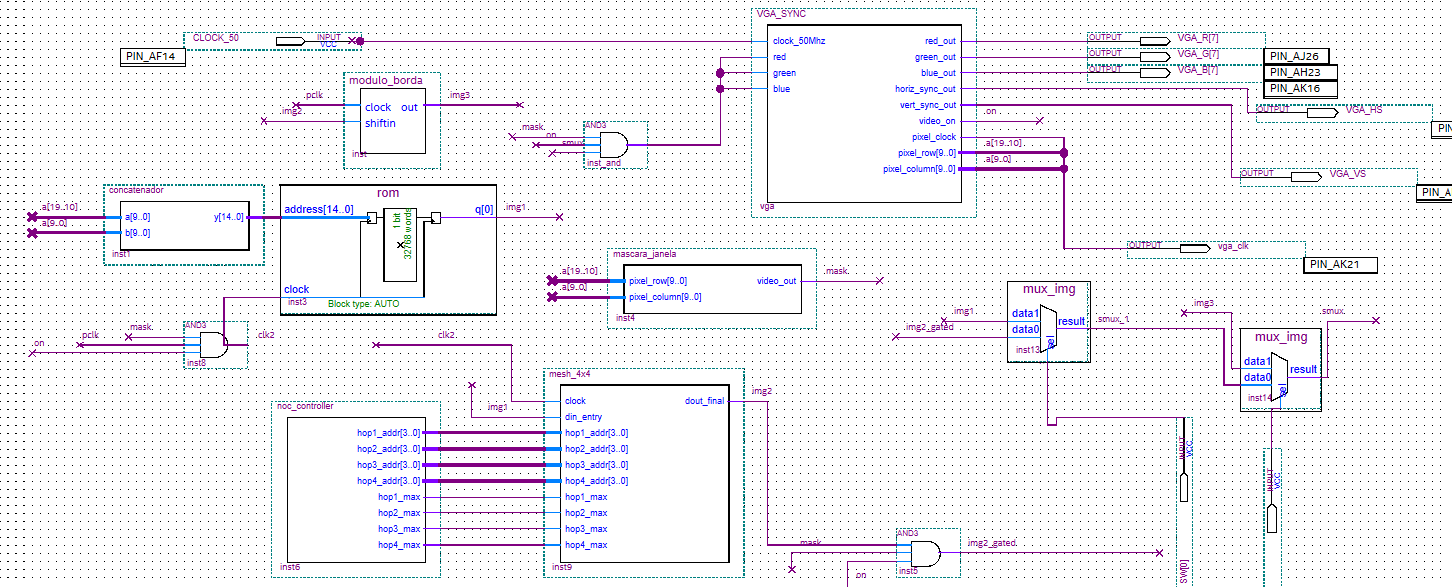
\includegraphics[width=1.0\textwidth]{top_bdf_entity_make_this_big_itishardtosee.png}
		\caption{Diagrama BDF do módulo \textit{top-level} \texttt{vga\_filtro}
			no Quartus Prime, evidenciando a interligação de todos os componentes
			do sistema de filtragem de imagem via rede \textit{mesh} 4$\times$4.}
		\label{fig:top_bdf}
	\end{figure}
	
	Os módulos que compõem o sistema são:
	
	\begin{itemize}
		\item \texttt{VGA\_SYNC} --- Controlador VGA (VHDL, fornecido); gera
		\texttt{HSync}, \texttt{VSync}, \texttt{video\_on}, \texttt{pixel\_clock}
		e os contadores de coordenadas \texttt{pixel\_column}/\texttt{pixel\_row};
		\item \texttt{rom} --- Memória ROM contendo a imagem original; endereçada
		pelo módulo \texttt{concatenador} com 15 bits de endereço;
		\item \texttt{concatenador} --- Módulo VHDL que forma o endereço de 15 bits
		da ROM a partir das coordenadas de pixel (\texttt{pixel\_row[6:0]} \&
		\texttt{pixel\_column[7:0]});
		\item \texttt{mascara\_janela} --- Módulo VHDL que delimita a região ativa
		de processamento (256$\times$128 pixels) e gera o sinal de máscara;
		\item \texttt{noc\_controller} --- Controlador estático da NoC; define os
		endereços e modos (máximo/mínimo) dos quatro nós do caminho ativo;
		\item \texttt{mesh\_4x4} --- Estrutura de interligação dos 16 nós
		\texttt{mesh\_node}, com toda a fiação de dados e sinais de validade;
		\item \texttt{mesh\_node} --- Nó elementar da rede; contém um roteador XY
		e um núcleo \texttt{modulo\_sal\_e\_pimenta};
		\item \texttt{modulo\_sal\_e\_pimenta} --- Núcleo de processamento de
		filtro sal e pimenta; composto por registradores de deslocamento de 256
		bits e módulo de máximo e mínimo de 9 bits;
		\item \texttt{modulo\_borda} --- Módulo de pós-processamento de borda
		(herdado da prática anterior), aplicado sobre a saída da \textit{mesh};
		\item \texttt{mux\_img} --- Multiplexador 2:1 para seleção de imagem
		exibida no VGA (original, filtrada, ou com borda), controlado por
		\texttt{SW[0]} e \texttt{SW[1]}.
	\end{itemize}
	
	\subsection{Módulo \texttt{concatenador} --- Formação do Endereço de ROM}
	
	O módulo \texttt{concatenador} é descrito em VHDL e realiza a concatenação
	das coordenadas de pixel para formar o endereço de 15 bits utilizado no acesso
	à ROM de imagem. Os 7 bits menos significativos da linha codificam as 128 linhas
	da imagem, enquanto os 8 bits menos significativos da coluna codificam as 256
	colunas, resultando em um espaço de endereçamento de $2^{15} = 32.768$ posições.
	
	\begin{lstlisting}[style=vhdl, caption={\texttt{concatenador.vhd} --- Concatenação de coordenadas de pixel para endereçamento da ROM de imagem.}, label={lst:concat}]
		library IEEE;
		use IEEE.STD_LOGIC_1164.ALL;
		entity concatenador is
		Port (
		a : in  STD_LOGIC_VECTOR(9 downto 0); -- linha
		b : in  STD_LOGIC_VECTOR(9 downto 0); -- coluna
		y : out STD_LOGIC_VECTOR(14 downto 0)
		);
		end concatenador;
		architecture Behavioral of concatenador is
		begin
		y <= a(6 downto 0) & b(7 downto 0);
		end Behavioral;
	\end{lstlisting}
	
	A entidade recebe os vetores de 10 bits \texttt{a} (linha) e \texttt{b}
	(coluna) e produz o vetor de saída \texttt{y} de 15 bits pela concatenação
	\texttt{a(6 downto 0) \& b(7 downto 0)}. Esta operação é puramente
	combinacional, sem registros intermediários, e é sintetizada como simples
	fios de conexão pelo Quartus Prime.
	
	\subsection{Módulo \texttt{mascara\_janela} --- Delimitação da Região Ativa}
	
	O módulo \texttt{mascara\_janela} delimita a região de interesse dentro do
	quadro VGA. Apenas a subjanela de 256 colunas por 128 linhas no canto
	superior esquerdo da tela é considerada ativa para processamento. O sinal
	\texttt{video\_out} é utilizado pelo \textit{top-level} para habilitar o
	clock da rede \textit{mesh} e para mascarar a saída final para o VGA.
	
	\begin{lstlisting}[style=vhdl, caption={\texttt{mascara\_janela.vhd} --- Geração do sinal de máscara para delimitação da região ativa de processamento.}, label={lst:mascara}]
		library IEEE;
		use IEEE.STD_LOGIC_1164.ALL;
		use IEEE.NUMERIC_STD.ALL;
		entity mascara_janela is
		Port (
		pixel_row    : in  STD_LOGIC_VECTOR(9 downto 0);
		pixel_column : in  STD_LOGIC_VECTOR(9 downto 0);
		video_out    : out STD_LOGIC
		);
		end mascara_janela;
		architecture Behavioral of mascara_janela is
		begin
		process(pixel_row, pixel_column)
		begin
		if (unsigned(pixel_column) < 256 and
		unsigned(pixel_row) < 128) then
		video_out <= '1';
		else
		video_out <= '0';
		end if;
		end process;
		end Behavioral;
	\end{lstlisting}
	
	O processo sensível às entradas \texttt{pixel\_row} e \texttt{pixel\_column}
	avalia as comparações sem sinal (\texttt{unsigned}) para evitar ambiguidade
	na interpretação do bit de sinal dos vetores \texttt{STD\_LOGIC\_VECTOR}.
	O resultado é uma lógica combinacional de dois comparadores de 10 bits em AND.
	
	\subsection{Módulo \texttt{modulo\_sal\_e\_pimenta} --- Núcleo de Processamento}
	
	O módulo \texttt{modulo\_sal\_e\_pimenta} implementa o filtro de ordem
	estatística sobre uma janela deslizante de $3\times3$ pixels em fluxo serial.
	Ele é gerado automaticamente pelo editor BDF do Quartus Prime e instancia três
	subcomponentes: dois registradores de deslocamento de 256 bits
	(\texttt{shift\_register}), um registrador de deslocamento de 3 bits
	(\texttt{shift\_3}) e o módulo de cálculo de máximo e mínimo sobre 9 bits
	(\texttt{max\_min\_9bits}).
	
	\begin{lstlisting}[style=verilog, caption={\texttt{modulo\_sal\_e\_pimenta.v} --- Núcleo de processamento do filtro sal e pimenta com janela $3\times3$ sobre fluxo serial de pixels.}, label={lst:salp}]
		module modulo_sal_e_pimenta(
		clock,
		shiftin,
		max_bit,
		min_bit
		);
		input wire  clock;
		input wire  shiftin;
		output wire max_bit;
		output wire min_bit;
		
		wire [255:0] q1;
		wire [255:0] q2;
		wire [2:0]   q3;
		
		shift_register b2v_inst(
		.clock(clock),
		.shiftin(shiftin),
		.q(q1));
		
		shift_register b2v_inst1(
		.clock(clock),
		.shiftin(q1[0]),
		.q(q2));
		
		max_min_9bits b2v_inst2(
		.in1(q1[255:253]),
		.in2(q2[255:253]),
		.in3(q3),
		.max_bit(max_bit),
		.min_bit(min_bit));
		
		shift_3 b2v_inst5(
		.clock(clock),
		.shiftin(q2[0]),
		.q(q3));
		
		endmodule
	\end{lstlisting}
	
	O funcionamento do módulo baseia-se na construção da janela $3\times3$ por
	meio de linhas de atraso em cascata. O pixel corrente entra em \texttt{shiftin}
	e é deslocado pelo primeiro registrador de 256 bits (\texttt{q1}), que modela
	uma linha de atraso de 256 pixels --- equivalente a um atraso de uma linha
	completa da imagem, uma vez que a região ativa tem 256 colunas. O bit de saída
	de \texttt{q1} (\texttt{q1[0]}) alimenta o segundo registrador de 256 bits
	(\texttt{q2}), modelando mais uma linha de atraso.
	
	Desta forma, em qualquer instante do processamento:
	
	\begin{itemize}
		\item \texttt{q1[255:253]}: os 3 pixels mais antigos da linha anterior
		(linha $y-1$, colunas $x-2$, $x-1$, $x$);
		\item \texttt{q2[255:253]}: os 3 pixels da linha anteanterior (linha $y-2$,
		colunas $x-2$, $x-1$, $x$);
		\item \texttt{q3[2:0]}: os 3 pixels mais recentes da linha atual (linha
		$y$, colunas $x-2$, $x-1$, $x$), fornecidos pelo registrador
		\texttt{shift\_3}.
	\end{itemize}
	
	Estes 9 bits --- três de cada uma das três linhas da janela --- são
	alimentados ao módulo \texttt{max\_min\_9bits}, que determina o bit de
	máximo (\texttt{max\_bit}) e o bit de mínimo (\texttt{min\_bit}) dentre os
	9 valores binários.
	
	\subsection{Módulo \texttt{mesh\_node} --- Nó Elementar da Rede}
	
	O módulo \texttt{mesh\_node} é o componente fundamental da rede
	\textit{mesh}. Ele combina a lógica de roteamento XY com o núcleo de
	processamento \texttt{modulo\_sal\_e\_pimenta}. O endereço do nó é definido
	pelo parâmetro estático \texttt{MY\_ADDR}, que determina sua posição na grade.
	
	\begin{lstlisting}[style=verilog, caption={\texttt{mesh\_node.v} --- Nó elementar da rede \textit{mesh} com roteador XY e núcleo de processamento de filtro sal e pimenta.}, label={lst:node}]
		module mesh_node #(
		parameter [3:0] MY_ADDR = 4'b0000
		)(
		input  wire        clock,
		input  wire [3:0]  hop1_addr, hop2_addr, hop3_addr, hop4_addr,
		input  wire        din_entry,
		input  wire        hop1_max, hop2_max, hop3_max, hop4_max,
		input  wire        din_n, din_s, din_e, din_w,
		input  wire        vin_n, vin_s, vin_e, vin_w,
		output wire        dout_n, dout_s, dout_e, dout_w,
		output wire        vout_n, vout_s, vout_e, vout_w,
		output wire        dout_final
		);
		localparam [1:0] my_col = MY_ADDR[3:2];
		localparam [1:0] my_row = MY_ADDR[1:0];
		
		// Verificacao de pertinencia ao caminho de processamento
		wire is_hop1 = (MY_ADDR == hop1_addr);
		wire is_hop2 = (MY_ADDR == hop2_addr);
		wire is_hop3 = (MY_ADDR == hop3_addr);
		wire is_hop4 = (MY_ADDR == hop4_addr);
		wire on_path = is_hop1 | is_hop2 | is_hop3 | is_hop4;
		
		// Determinacao do proximo salto
		wire [3:0] next_addr = is_hop1 ? hop2_addr :
		is_hop2 ? hop3_addr :
		is_hop3 ? hop4_addr :
		hop4_addr;
		wire [1:0] next_col = next_addr[3:2];
		wire [1:0] next_row = next_addr[1:0];
		
		// Decisoes de roteamento XY
		wire go_s = on_path && !is_hop4 && (my_row < next_row);
		wire go_n = on_path && !is_hop4 && (my_row > next_row);
		wire go_e = on_path && !is_hop4 && (my_row == next_row)
		&& (my_col < next_col);
		wire go_w = on_path && !is_hop4 && (my_row == next_row)
		&& (my_col > next_col);
		
		// Selecao do dado de entrada via sinais de validade
		wire data_in = vin_n ? din_n :
		vin_s ? din_s :
		vin_e ? din_e :
		vin_w ? din_w :
		1'b0;
		
		// Entrada do nucleo de processamento
		wire pe_in = is_hop1 ? din_entry : data_in;
		
		wire pe_max_out, pe_min_out;
		modulo_sal_e_pimenta u_pe (
		.clock   (clock),
		.shiftin (pe_in),
		.max_bit (pe_max_out),
		.min_bit (pe_min_out)
		);
		
		// Selecao de modo (maximo ou minimo) por salto
		wire my_max = is_hop1 ? hop1_max :
		is_hop2 ? hop2_max :
		is_hop3 ? hop3_max :
		hop4_max;
		wire pe_out = my_max ? pe_max_out : pe_min_out;
		
		// Dado encaminhado: resultado do PE (no caminho) ou retransmissao
		wire fwd = on_path ? pe_out : data_in;
		
		// Saidas direcionais
		assign dout_s = go_s ? fwd : 1'b0;
		assign dout_n = go_n ? fwd : 1'b0;
		assign dout_e = go_e ? fwd : 1'b0;
		assign dout_w = go_w ? fwd : 1'b0;
		
		// Sinais de validade de saida
		assign vout_s = go_s;
		assign vout_n = go_n;
		assign vout_e = go_e;
		assign vout_w = go_w;
		
		// Saida final: apenas o no de destino (hop4) expoe o resultado
		assign dout_final = is_hop4 ? pe_out : 1'b0;
		endmodule
	\end{lstlisting}
	
	O módulo opera da seguinte forma. Primeiramente, os sinais \texttt{is\_hop1}
	a \texttt{is\_hop4} determinam se este nó faz parte do caminho de
	processamento e, em caso afirmativo, qual é seu papel (entrada, intermediário
	ou destino). O sinal \texttt{on\_path} é a disjunção dos quatro.
	
	Em seguida, \texttt{next\_addr} identifica o endereço do próximo nó no
	caminho: se o nó atual é \texttt{hop1}, o próximo é \texttt{hop2}; se é
	\texttt{hop2}, o próximo é \texttt{hop3}; e assim por diante. Para
	\texttt{hop4} (destino), não há próximo nó relevante, e as decisões de
	roteamento são inibidas pela condição \texttt{!is\_hop4}.
	
	As decisões de roteamento (\texttt{go\_s}, \texttt{go\_n}, \texttt{go\_e},
	\texttt{go\_w}) comparam a posição do nó atual com a do próximo, implementando
	o roteamento determinístico. A prioridade das condições de linha sobre as de
	coluna realiza efetivamente uma política YX (vertical primeiro, depois
	horizontal).
	
	O dado de entrada ao núcleo de processamento (\texttt{pe\_in}) é selecionado
	pelo multiplexador de entrada: para \texttt{hop1}, é o dado externo
	\texttt{din\_entry}; para os demais, é o dado recebido de um vizinho válido
	(\texttt{data\_in}), selecionado pelo sinal de validade mais prioritário entre
	os quatro vizinhos.
	
	O núcleo \texttt{modulo\_sal\_e\_pimenta} processa \texttt{pe\_in} e produz
	\texttt{pe\_max\_out} e \texttt{pe\_min\_out}. O sinal \texttt{my\_max}
	seleciona qual dos dois é o resultado efetivo \texttt{pe\_out} para este nó,
	baseando-se nos bits de modo fornecidos pelo \texttt{noc\_controller}.
	
	Por fim, o dado encaminhado (\texttt{fwd}) é o resultado do PE se o nó está
	no caminho, ou simplesmente o dado recebido (\texttt{data\_in}) se o nó é
	apenas roteador. As saídas direcionais são atribuídas condicionalmente às
	decisões de roteamento, e o sinal \texttt{dout\_final} só é assertado pelo
	nó de destino (\texttt{is\_hop4}).
	
	\subsection{Módulo \texttt{mesh\_4x4} --- Interligação da Rede}
	
	O módulo \texttt{mesh\_4x4} instancia os 16 nós \texttt{mesh\_node} e realiza
	toda a fiação de dados e sinais de validade entre os vizinhos na topologia
	\textit{mesh} 4$\times$4. A saída \texttt{dout\_final} é o OR lógico das
	saídas individuais dos 16 nós --- como apenas o nó de destino (\texttt{hop4})
	assertará \texttt{dout\_final} com valor não nulo, o OR efetivamente propaga
	apenas o resultado do processamento.
	
	\begin{lstlisting}[style=verilog, caption={\texttt{mesh\_4x4.v} --- Estrutura de interligação dos 16 nós da rede \textit{mesh} 4$\times$4, com fiação completa de dados e sinais de validade.}, label={lst:mesh4x4}]
		module mesh_4x4 (
		input  wire        clock,
		input  wire        din_entry,
		input  wire [3:0]  hop1_addr, hop2_addr, hop3_addr, hop4_addr,
		input  wire        hop1_max, hop2_max, hop3_max, hop4_max,
		output wire        dout_final
		);
		// --- Wires de dados na direcao leste ---
		wire e_00, e_10, e_20;
		wire e_01, e_11, e_21;
		wire e_02, e_12, e_22;
		wire e_03, e_13, e_23;
		
		// --- Wires de dados na direcao sul ---
		wire s_00, s_10, s_20, s_30;
		wire s_01, s_11, s_21, s_31;
		wire s_02, s_12, s_22, s_32;
		
		// --- Wires de dados na direcao norte ---
		wire n_01, n_11, n_21, n_31;
		wire n_02, n_12, n_22, n_32;
		wire n_03, n_13, n_23, n_33;
		
		// --- Wires de validade na direcao leste ---
		wire ve_00, ve_10, ve_20;
		wire ve_01, ve_11, ve_21;
		wire ve_02, ve_12, ve_22;
		wire ve_03, ve_13, ve_23;
		
		// --- Wires de validade na direcao sul ---
		wire vs_00, vs_10, vs_20, vs_30;
		wire vs_01, vs_11, vs_21, vs_31;
		wire vs_02, vs_12, vs_22, vs_32;
		
		// --- Wires de validade na direcao norte ---
		wire vn_01, vn_11, vn_21, vn_31;
		wire vn_02, vn_12, vn_22, vn_32;
		wire vn_03, vn_13, vn_23, vn_33;
		
		// --- Wires de saida final por no ---
		wire r_00, r_10, r_20, r_30;
		wire r_01, r_11, r_21, r_31;
		wire r_02, r_12, r_22, r_32;
		wire r_03, r_13, r_23, r_33;
		
		// --- Linha 0 (row=0): n00, n10, n20, n30 ---
		mesh_node #(.MY_ADDR(4'b0000)) n00 ( .clock(clock),
		.hop1_addr(hop1_addr),.hop2_addr(hop2_addr),
		.hop3_addr(hop3_addr),.hop4_addr(hop4_addr),
		.hop1_max(hop1_max),.hop2_max(hop2_max),
		.hop3_max(hop3_max),.hop4_max(hop4_max),
		.din_entry(din_entry),
		.din_n(1'b0),.din_s(n_01),.din_e(e_10),.din_w(1'b0),
		.vin_n(1'b0),.vin_s(vn_01),.vin_e(ve_10),.vin_w(1'b0),
		.dout_n(),.dout_s(s_00),.dout_e(e_00),.dout_w(),
		.vout_n(),.vout_s(vs_00),.vout_e(ve_00),.vout_w(),
		.dout_final(r_00));
		
		mesh_node #(.MY_ADDR(4'b0100)) n10 ( .clock(clock),
		.hop1_addr(hop1_addr),.hop2_addr(hop2_addr),
		.hop3_addr(hop3_addr),.hop4_addr(hop4_addr),
		.hop1_max(hop1_max),.hop2_max(hop2_max),
		.hop3_max(hop3_max),.hop4_max(hop4_max),
		.din_entry(din_entry),
		.din_n(1'b0),.din_s(n_11),.din_e(e_20),.din_w(e_00),
		.vin_n(1'b0),.vin_s(vn_11),.vin_e(ve_20),.vin_w(ve_00),
		.dout_n(),.dout_s(s_10),.dout_e(e_10),.dout_w(),
		.vout_n(),.vout_s(vs_10),.vout_e(ve_10),.vout_w(),
		.dout_final(r_10));
		
		mesh_node #(.MY_ADDR(4'b1000)) n20 ( .clock(clock),
		.hop1_addr(hop1_addr),.hop2_addr(hop2_addr),
		.hop3_addr(hop3_addr),.hop4_addr(hop4_addr),
		.hop1_max(hop1_max),.hop2_max(hop2_max),
		.hop3_max(hop3_max),.hop4_max(hop4_max),
		.din_entry(din_entry),
		.din_n(1'b0),.din_s(n_21),.din_e(1'b0),.din_w(e_10),
		.vin_n(1'b0),.vin_s(vn_21),.vin_e(1'b0),.vin_w(ve_10),
		.dout_n(),.dout_s(s_20),.dout_e(e_20),.dout_w(),
		.vout_n(),.vout_s(vs_20),.vout_e(ve_20),.vout_w(),
		.dout_final(r_20));
		
		mesh_node #(.MY_ADDR(4'b1100)) n30 ( .clock(clock),
		.hop1_addr(hop1_addr),.hop2_addr(hop2_addr),
		.hop3_addr(hop3_addr),.hop4_addr(hop4_addr),
		.hop1_max(hop1_max),.hop2_max(hop2_max),
		.hop3_max(hop3_max),.hop4_max(hop4_max),
		.din_entry(din_entry),
		.din_n(1'b0),.din_s(n_31),.din_e(1'b0),.din_w(e_20),
		.vin_n(1'b0),.vin_s(vn_31),.vin_e(1'b0),.vin_w(ve_20),
		.dout_n(),.dout_s(s_30),.dout_e(),.dout_w(),
		.vout_n(),.vout_s(vs_30),.vout_e(),.vout_w(),
		.dout_final(r_30));
		
		// --- Linha 1 (row=1): n01, n11, n21, n31 ---
		mesh_node #(.MY_ADDR(4'b0001)) n01 ( .clock(clock),
		.hop1_addr(hop1_addr),.hop2_addr(hop2_addr),
		.hop3_addr(hop3_addr),.hop4_addr(hop4_addr),
		.hop1_max(hop1_max),.hop2_max(hop2_max),
		.hop3_max(hop3_max),.hop4_max(hop4_max),
		.din_entry(din_entry),
		.din_n(s_00),.din_s(n_02),.din_e(e_11),.din_w(1'b0),
		.vin_n(vs_00),.vin_s(vn_02),.vin_e(ve_11),.vin_w(1'b0),
		.dout_n(n_01),.dout_s(s_01),.dout_e(e_01),.dout_w(),
		.vout_n(vn_01),.vout_s(vs_01),.vout_e(ve_01),.vout_w(),
		.dout_final(r_01));
		
		mesh_node #(.MY_ADDR(4'b0101)) n11 ( .clock(clock),
		.hop1_addr(hop1_addr),.hop2_addr(hop2_addr),
		.hop3_addr(hop3_addr),.hop4_addr(hop4_addr),
		.hop1_max(hop1_max),.hop2_max(hop2_max),
		.hop3_max(hop3_max),.hop4_max(hop4_max),
		.din_entry(din_entry),
		.din_n(s_10),.din_s(n_12),.din_e(e_21),.din_w(e_01),
		.vin_n(vs_10),.vin_s(vn_12),.vin_e(ve_21),.vin_w(ve_01),
		.dout_n(n_11),.dout_s(s_11),.dout_e(e_11),.dout_w(),
		.vout_n(vn_11),.vout_s(vs_11),.vout_e(ve_11),.vout_w(),
		.dout_final(r_11));
		
		mesh_node #(.MY_ADDR(4'b1001)) n21 ( .clock(clock),
		.hop1_addr(hop1_addr),.hop2_addr(hop2_addr),
		.hop3_addr(hop3_addr),.hop4_addr(hop4_addr),
		.hop1_max(hop1_max),.hop2_max(hop2_max),
		.hop3_max(hop3_max),.hop4_max(hop4_max),
		.din_entry(din_entry),
		.din_n(s_20),.din_s(n_22),.din_e(1'b0),.din_w(e_11),
		.vin_n(vs_20),.vin_s(vn_22),.vin_e(1'b0),.vin_w(ve_11),
		.dout_n(n_21),.dout_s(s_21),.dout_e(e_21),.dout_w(),
		.vout_n(vn_21),.vout_s(vs_21),.vout_e(ve_21),.vout_w(),
		.dout_final(r_21));
		
		mesh_node #(.MY_ADDR(4'b1101)) n31 ( .clock(clock),
		.hop1_addr(hop1_addr),.hop2_addr(hop2_addr),
		.hop3_addr(hop3_addr),.hop4_addr(hop4_addr),
		.hop1_max(hop1_max),.hop2_max(hop2_max),
		.hop3_max(hop3_max),.hop4_max(hop4_max),
		.din_entry(din_entry),
		.din_n(s_30),.din_s(n_32),.din_e(1'b0),.din_w(e_21),
		.vin_n(vs_30),.vin_s(vn_32),.vin_e(1'b0),.vin_w(ve_21),
		.dout_n(n_31),.dout_s(s_31),.dout_e(),.dout_w(),
		.vout_n(vn_31),.vout_s(vs_31),.vout_e(),.vout_w(),
		.dout_final(r_31));
		
		// --- Linha 2 (row=2): n02, n12, n22, n32 ---
		mesh_node #(.MY_ADDR(4'b0010)) n02 ( .clock(clock),
		.hop1_addr(hop1_addr),.hop2_addr(hop2_addr),
		.hop3_addr(hop3_addr),.hop4_addr(hop4_addr),
		.hop1_max(hop1_max),.hop2_max(hop2_max),
		.hop3_max(hop3_max),.hop4_max(hop4_max),
		.din_entry(din_entry),
		.din_n(s_01),.din_s(n_03),.din_e(e_12),.din_w(1'b0),
		.vin_n(vs_01),.vin_s(vn_03),.vin_e(ve_12),.vin_w(1'b0),
		.dout_n(n_02),.dout_s(s_02),.dout_e(e_02),.dout_w(),
		.vout_n(vn_02),.vout_s(vs_02),.vout_e(ve_02),.vout_w(),
		.dout_final(r_02));
		
		mesh_node #(.MY_ADDR(4'b0110)) n12 ( .clock(clock),
		.hop1_addr(hop1_addr),.hop2_addr(hop2_addr),
		.hop3_addr(hop3_addr),.hop4_addr(hop4_addr),
		.hop1_max(hop1_max),.hop2_max(hop2_max),
		.hop3_max(hop3_max),.hop4_max(hop4_max),
		.din_entry(din_entry),
		.din_n(s_11),.din_s(n_13),.din_e(e_22),.din_w(e_02),
		.vin_n(vs_11),.vin_s(vn_13),.vin_e(ve_22),.vin_w(ve_02),
		.dout_n(n_12),.dout_s(s_12),.dout_e(e_12),.dout_w(),
		.vout_n(vn_12),.vout_s(vs_12),.vout_e(ve_12),.vout_w(),
		.dout_final(r_12));
		
		mesh_node #(.MY_ADDR(4'b1010)) n22 ( .clock(clock),
		.hop1_addr(hop1_addr),.hop2_addr(hop2_addr),
		.hop3_addr(hop3_addr),.hop4_addr(hop4_addr),
		.hop1_max(hop1_max),.hop2_max(hop2_max),
		.hop3_max(hop3_max),.hop4_max(hop4_max),
		.din_entry(din_entry),
		.din_n(s_21),.din_s(n_23),.din_e(1'b0),.din_w(e_12),
		.vin_n(vs_21),.vin_s(vn_23),.vin_e(1'b0),.vin_w(ve_12),
		.dout_n(n_22),.dout_s(s_22),.dout_e(e_22),.dout_w(),
		.vout_n(vn_22),.vout_s(vs_22),.vout_e(ve_22),.vout_w(),
		.dout_final(r_22));
		
		mesh_node #(.MY_ADDR(4'b1110)) n32 ( .clock(clock),
		.hop1_addr(hop1_addr),.hop2_addr(hop2_addr),
		.hop3_addr(hop3_addr),.hop4_addr(hop4_addr),
		.hop1_max(hop1_max),.hop2_max(hop2_max),
		.hop3_max(hop3_max),.hop4_max(hop4_max),
		.din_entry(din_entry),
		.din_n(s_31),.din_s(n_33),.din_e(1'b0),.din_w(e_22),
		.vin_n(vs_31),.vin_s(vn_33),.vin_e(1'b0),.vin_w(ve_22),
		.dout_n(n_32),.dout_s(s_32),.dout_e(),.dout_w(),
		.vout_n(vn_32),.vout_s(vs_32),.vout_e(),.vout_w(),
		.dout_final(r_32));
		
		// --- Linha 3 (row=3): n03, n13, n23, n33 ---
		mesh_node #(.MY_ADDR(4'b0011)) n03 ( .clock(clock),
		.hop1_addr(hop1_addr),.hop2_addr(hop2_addr),
		.hop3_addr(hop3_addr),.hop4_addr(hop4_addr),
		.hop1_max(hop1_max),.hop2_max(hop2_max),
		.hop3_max(hop3_max),.hop4_max(hop4_max),
		.din_entry(din_entry),
		.din_n(s_02),.din_s(1'b0),.din_e(e_13),.din_w(1'b0),
		.vin_n(vs_02),.vin_s(1'b0),.vin_e(ve_13),.vin_w(1'b0),
		.dout_n(n_03),.dout_s(),.dout_e(e_03),.dout_w(),
		.vout_n(vn_03),.vout_s(),.vout_e(ve_03),.vout_w(),
		.dout_final(r_03));
		
		mesh_node #(.MY_ADDR(4'b0111)) n13 ( .clock(clock),
		.hop1_addr(hop1_addr),.hop2_addr(hop2_addr),
		.hop3_addr(hop3_addr),.hop4_addr(hop4_addr),
		.hop1_max(hop1_max),.hop2_max(hop2_max),
		.hop3_max(hop3_max),.hop4_max(hop4_max),
		.din_entry(din_entry),
		.din_n(s_12),.din_s(1'b0),.din_e(e_23),.din_w(e_03),
		.vin_n(vs_12),.vin_s(1'b0),.vin_e(ve_23),.vin_w(ve_03),
		.dout_n(n_13),.dout_s(),.dout_e(e_13),.dout_w(),
		.vout_n(vn_13),.vout_s(),.vout_e(ve_13),.vout_w(),
		.dout_final(r_13));
		
		mesh_node #(.MY_ADDR(4'b1011)) n23 ( .clock(clock),
		.hop1_addr(hop1_addr),.hop2_addr(hop2_addr),
		.hop3_addr(hop3_addr),.hop4_addr(hop4_addr),
		.hop1_max(hop1_max),.hop2_max(hop2_max),
		.hop3_max(hop3_max),.hop4_max(hop4_max),
		.din_entry(din_entry),
		.din_n(s_22),.din_s(1'b0),.din_e(1'b0),.din_w(e_13),
		.vin_n(vs_22),.vin_s(1'b0),.vin_e(1'b0),.vin_w(ve_13),
		.dout_n(n_23),.dout_s(),.dout_e(e_23),.dout_w(),
		.vout_n(vn_23),.vout_s(),.vout_e(ve_23),.vout_w(),
		.dout_final(r_23));
		
		mesh_node #(.MY_ADDR(4'b1111)) n33 ( .clock(clock),
		.hop1_addr(hop1_addr),.hop2_addr(hop2_addr),
		.hop3_addr(hop3_addr),.hop4_addr(hop4_addr),
		.hop1_max(hop1_max),.hop2_max(hop2_max),
		.hop3_max(hop3_max),.hop4_max(hop4_max),
		.din_entry(din_entry),
		.din_n(s_32),.din_s(1'b0),.din_e(1'b0),.din_w(e_23),
		.vin_n(vs_32),.vin_s(1'b0),.vin_e(1'b0),.vin_w(ve_23),
		.dout_n(n_33),.dout_s(),.dout_e(),.dout_w(),
		.vout_n(vn_33),.vout_s(),.vout_e(),.vout_w(),
		.dout_final(r_33));
		
		// Saida final: OR de todos os nos (apenas hop4 assertara)
		assign dout_final =
		r_00 | r_10 | r_20 | r_30 |
		r_01 | r_11 | r_21 | r_31 |
		r_02 | r_12 | r_22 | r_32 |
		r_03 | r_13 | r_23 | r_33;
		
		endmodule
	\end{lstlisting}
	
	A fiação do módulo segue uma nomenclatura sistemática: os fios de dados na
	direção leste são denominados \texttt{e\_CR} (onde \texttt{C} é a coluna de
	origem e \texttt{R} é a linha), os fios na direção sul são \texttt{s\_CR}, e
	os fios na direção norte são \texttt{n\_CR}. Os fios de validade correspondentes
	recebem o prefixo \texttt{v} (\texttt{ve\_CR}, \texttt{vs\_CR}, \texttt{vn\_CR}).
	Os fios de saída final individual de cada nó são \texttt{r\_CR}.
	
	A lógica de interligação é direta: a saída \texttt{dout\_s} do nó $(col, row)$
	conecta-se à entrada \texttt{din\_n} do nó $(col, row+1)$, e reciprocamente a
	saída \texttt{dout\_n} de $(col, row)$ conecta-se à entrada \texttt{din\_s}
	de $(col, row-1)$. Analogamente para as direções leste e oeste. As fronteiras
	da \textit{mesh} são conectadas a \texttt{1'b0} (dado) e \texttt{1'b0}
	(validade), indicando ausência de vizinho externo.
	
	\subsection{Módulo \texttt{noc\_controller} --- Configuração do Caminho Ativo}
	
	O módulo \texttt{noc\_controller} define estaticamente o caminho de
	processamento ativo na rede \textit{mesh}, especificando os endereços dos
	quatro nós do caminho e o modo de operação (máximo ou mínimo) de cada um.
	Trata-se de um módulo puramente combinacional, sem clock, com saídas
	constantes determinadas em tempo de elaboração.
	
	\begin{lstlisting}[style=verilog, caption={\texttt{noc\_controller.v} --- Controlador estático do caminho de processamento da NoC, com três configurações de roteamento disponíveis.}, label={lst:noc}]
		module noc_controller (
		output wire [3:0] hop1_addr,
		output wire [3:0] hop2_addr,
		output wire [3:0] hop3_addr,
		output wire [3:0] hop4_addr,
		output wire       hop1_max,
		output wire       hop2_max,
		output wire       hop3_max,
		output wire       hop4_max
		);
		// Configuracao 1: Coluna Vertical (col=1, linhas 0->3)
		// assign hop1_addr = 4'b0100; assign hop1_max = 1'b1; // n10 MAX
		// assign hop2_addr = 4'b0101; assign hop2_max = 1'b0; // n11 MIN
		// assign hop3_addr = 4'b0110; assign hop3_max = 1'b0; // n12 MIN
		// assign hop4_addr = 4'b0111; assign hop4_max = 1'b1; // n13 MAX
		
		// Configuracao 2: Quatro juntos no topo (L superior esquerdo)
		// assign hop1_addr = 4'b0000; assign hop1_max = 1'b1; // n00 MAX
		// assign hop2_addr = 4'b0001; assign hop2_max = 1'b0; // n01 MIN
		// assign hop3_addr = 4'b0101; assign hop3_max = 1'b0; // n11 MIN
		// assign hop4_addr = 4'b0110; assign hop4_max = 1'b1; // n12 MAX
		
		// Configuracao 3: Diagonal (ativa)
		assign hop1_addr = 4'b0101; assign hop1_max = 1'b1; // n11 MAX
		assign hop2_addr = 4'b0110; assign hop2_max = 1'b0; // n12 MIN
		assign hop3_addr = 4'b1010; assign hop3_max = 1'b0; // n22 MIN
		assign hop4_addr = 4'b1011; assign hop4_max = 1'b1; // n23 MAX
		
		endmodule
	\end{lstlisting}
	
	Na configuração diagonal ativa, o caminho percorre os nós n11
	$\to$ n12 $\to$ n22 $\to$ n23. O roteamento XY entre os nós é:
	
	\begin{itemize}
		\item \textbf{n11 $\to$ n12}: mesma coluna (col=1), linha aumenta de 1
		para 2 $\Rightarrow$ \texttt{go\_s = 1};
		\item \textbf{n12 $\to$ n22}: mesma linha (row=2), coluna aumenta de 1
		para 2 $\Rightarrow$ \texttt{go\_e = 1};
		\item \textbf{n22 $\to$ n23}: mesma coluna (col=2), linha aumenta de 2
		para 3 $\Rightarrow$ \texttt{go\_s = 1}.
	\end{itemize}
	
	A sequência de modos é MAX $\to$ MIN $\to$ MIN $\to$ MAX, implementando um
	filtro composto que aplica dilatação seguida de erosão (equivalente a uma
	abertura morfológica) e depois erosão seguida de dilatação nos dois nós finais.
	
	\subsection{Módulo \textit{Top-Level} \texttt{vga\_filtro}}
	
	O módulo \textit{top-level} \texttt{vga\_filtro} integra todos os componentes
	e define o fluxo de sinal completo, desde a leitura da ROM até a exibição
	no monitor VGA. A Tabela~\ref{tab:controles} descreve o mapeamento das
	entradas de controle disponíveis ao usuário.
	
	\begin{table}[H]
		\centering
		\caption{Mapeamento de entradas de controle da placa DE1.}
		\label{tab:controles}
		\begin{tabular}{lll}
			\toprule
			\textbf{Pino} & \textbf{Sinal} & \textbf{Função} \\
			\midrule
			\texttt{SW[0]} & \texttt{sel (mux\_img inst13)} & 1 = original; 0 = filtrada/borda \\
			\texttt{SW[1]} & \texttt{sel (mux\_img inst14)} & 1 = borda; 0 = seleção de SW[0]  \\
			\bottomrule
		\end{tabular}
	\end{table}
	
	\begin{lstlisting}[style=verilog, caption={\texttt{vga\_filtro.v} --- Módulo \textit{top-level} gerado pelo editor BDF do Quartus Prime, integrando todos os componentes do sistema de filtragem via \textit{mesh}.}, label={lst:top}]
		module vga_filtro(
		CLOCK_50,
		SW,
		VGA_HS,
		VGA_VS,
		vga_clk,
		VGA_B,
		VGA_G,
		VGA_R
		);
		input wire        CLOCK_50;
		input wire  [1:0] SW;
		output wire       VGA_HS;
		output wire       VGA_VS;
		output wire       vga_clk;
		output wire [7:7] VGA_B;
		output wire [7:7] VGA_G;
		output wire [7:7] VGA_R;
		
		wire [19:0] a;          // {pixel_row[9:0], pixel_column[9:0]}
		wire        clk2;       // clock gated para a mesh
		wire        img1;       // pixel da ROM (imagem original)
		wire        img2;       // pixel filtrado pela mesh
		wire        img2_gated; // img2 mascarado para a regiao ativa
		wire        img3;       // pixel apos modulo_borda
		wire        mask;       // mascara da janela ativa
		wire        on;         // video_on do VGA
		wire        pclk;       // pixel clock VGA (~25 MHz)
		wire        smux;       // saida do segundo mux (para VGA)
		wire        smux_1;     // saida do primeiro mux
		
		wire [14:0] SYNTHESIZED_WIRE_0;  // endereco da ROM
		wire        SYNTHESIZED_WIRE_1;  // hop1_max
		wire        SYNTHESIZED_WIRE_2;  // hop2_max
		wire        SYNTHESIZED_WIRE_3;  // hop3_max
		wire        SYNTHESIZED_WIRE_4;  // hop4_max
		wire  [3:0] SYNTHESIZED_WIRE_5;  // hop1_addr
		wire  [3:0] SYNTHESIZED_WIRE_6;  // hop2_addr
		wire  [3:0] SYNTHESIZED_WIRE_7;  // hop3_addr
		wire  [3:0] SYNTHESIZED_WIRE_8;  // hop4_addr
		wire        SYNTHESIZED_WIRE_12; // pixel final para o VGA
		
		// Modulo de borda sobre a saida da mesh
		modulo_borda b2v_inst(
		.clock(pclk),
		.shiftin(img2),
		.out(img3));
		
		// Formacao do endereco de 15 bits para a ROM
		concatenador b2v_inst1(
		.a(a[19:10]),
		.b(a[9:0]),
		.y(SYNTHESIZED_WIRE_0));
		
		// Mux 1: seleciona entre original (img1) e filtrada (img2_gated)
		mux_img b2v_inst13(
		.data1(img1),
		.data0(img2_gated),
		.sel(SW[0]),
		.result(smux_1));
		
		// Mux 2: seleciona entre borda (img3) e saida do mux1
		mux_img b2v_inst14(
		.data1(img3),
		.data0(smux_1),
		.sel(SW[1]),
		.result(smux));
		
		// ROM de imagem: clock gated, 15 bits de endereco, 1 bit de saida
		rom b2v_inst3(
		.clock(clk2),
		.address(SYNTHESIZED_WIRE_0),
		.q(img1));
		
		// Mascara da janela ativa (256x128 pixels)
		mascara_janela b2v_inst4(
		.pixel_column(a[9:0]),
		.pixel_row(a[19:10]),
		.video_out(mask));
		
		// Img2 mascarado: apenas pixels validos da regiao ativa
		assign img2_gated = img2 & mask & on;
		
		// Controlador estatico da NoC
		noc_controller b2v_inst6(
		.hop1_max(SYNTHESIZED_WIRE_1),
		.hop2_max(SYNTHESIZED_WIRE_2),
		.hop3_max(SYNTHESIZED_WIRE_3),
		.hop4_max(SYNTHESIZED_WIRE_4),
		.hop1_addr(SYNTHESIZED_WIRE_5),
		.hop2_addr(SYNTHESIZED_WIRE_6),
		.hop3_addr(SYNTHESIZED_WIRE_7),
		.hop4_addr(SYNTHESIZED_WIRE_8));
		
		// Clock gated: ativo apenas na regiao de imagem valida
		assign clk2 = mask & pclk & on;
		
		// Rede mesh 4x4
		mesh_4x4 b2v_inst9(
		.clock(clk2),
		.din_entry(img1),
		.hop1_max(SYNTHESIZED_WIRE_1),
		.hop2_max(SYNTHESIZED_WIRE_2),
		.hop3_max(SYNTHESIZED_WIRE_3),
		.hop4_max(SYNTHESIZED_WIRE_4),
		.hop1_addr(SYNTHESIZED_WIRE_5),
		.hop2_addr(SYNTHESIZED_WIRE_6),
		.hop3_addr(SYNTHESIZED_WIRE_7),
		.hop4_addr(SYNTHESIZED_WIRE_8),
		.dout_final(img2));
		
		// Pixel final: mascarado pela janela e pelo video_on
		assign SYNTHESIZED_WIRE_12 = mask & on & smux;
		
		// Controlador VGA (VHDL, fornecido pelo professor)
		VGA_SYNC b2v_vga(
		.clock_50Mhz(CLOCK_50),
		.red(SYNTHESIZED_WIRE_12),
		.green(SYNTHESIZED_WIRE_12),
		.blue(SYNTHESIZED_WIRE_12),
		.red_out(VGA_R),
		.green_out(VGA_G),
		.blue_out(VGA_B),
		.horiz_sync_out(VGA_HS),
		.vert_sync_out(VGA_VS),
		.video_on(on),
		.pixel_clock(pclk),
		.pixel_column(a[9:0]),
		.pixel_row(a[19:10]));
		
		assign vga_clk = pclk;
		
		endmodule
	\end{lstlisting}
	
	O fluxo de dados no \textit{top-level} é o seguinte. O controlador VGA gera
	continuamente as coordenadas de pixel (\texttt{a[9:0]} para coluna,
	\texttt{a[19:10]} para linha) e os sinais de sincronismo. O módulo
	\texttt{concatenador} transforma essas coordenadas no endereço de 15 bits
	para a ROM. O módulo \texttt{mascara\_janela} determina se o pixel corrente
	está dentro da região ativa de $256\times128$ pixels.
	
	O clock gated \texttt{clk2} é formado pelo AND de \texttt{mask}, \texttt{pclk}
	e \texttt{on}, garantindo que a ROM e a rede \textit{mesh} avancem somente
	quando há um pixel ativo sendo processado. Isso é crucial para que os
	registradores de deslocamento internos ao \texttt{modulo\_sal\_e\_pimenta}
	contem corretamente os pixels da imagem.
	
	O pixel lido da ROM (\texttt{img1}) é injetado diretamente na rede
	\textit{mesh} (\texttt{din\_entry}), que produz o pixel filtrado
	(\texttt{img2}). O sinal \texttt{img2\_gated} é o pixel filtrado mascarado,
	utilizado como uma das entradas do primeiro multiplexador. O módulo
	\texttt{modulo\_borda} aplica um filtro de detecção de borda sobre \texttt{img2}
	para produzir \texttt{img3}. Os dois multiplexadores permitem ao usuário
	selecionar, via \texttt{SW[0]} e \texttt{SW[1]}, qual das três imagens
	(original, filtrada ou com borda) é exibida no VGA.
	
	\subsection{Diagramas BDF dos Componentes}
	
	A Figura~\ref{fig:rom_bdf} apresenta o diagrama BDF da memória ROM de
	imagem no Quartus Prime.
	
	\begin{figure}[H]
		\centering
		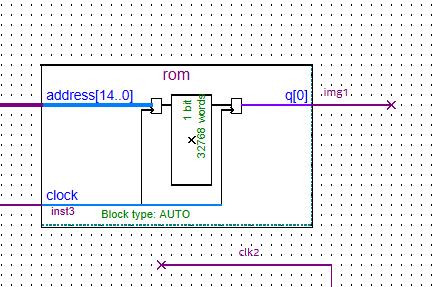
\includegraphics[width=0.70\textwidth]{rom_in_bdf.png}
		\caption{Diagrama BDF do módulo \texttt{rom} no Quartus Prime, com clock
			gated, endereço de 15 bits e saída de 1 bit por ciclo.}
		\label{fig:rom_bdf}
	\end{figure}
	
	A Figura~\ref{fig:vga_bdf} apresenta o diagrama BDF do controlador VGA
	integrado ao \textit{top-level}.
	
	\begin{figure}[H]
		\centering
		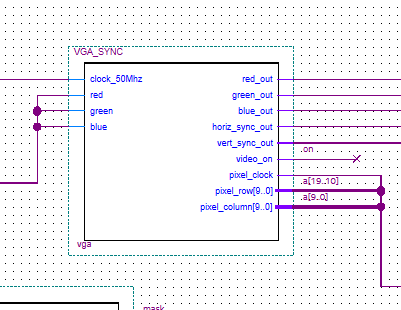
\includegraphics[width=0.90\textwidth]{vga_sync_intopbdf.png}
		\caption{Diagrama BDF do controlador \texttt{VGA\_SYNC} no \textit{top-level},
			evidenciando as saídas de sincronismo, pixel clock, coordenadas de
			varredura e sinal \texttt{video\_on}.}
		\label{fig:vga_bdf}
	\end{figure}
	
	A Figura~\ref{fig:mux_bdf} apresenta os multiplexadores de seleção de imagem
	reutilizados da prática anterior.
	
	\begin{figure}[H]
		\centering
		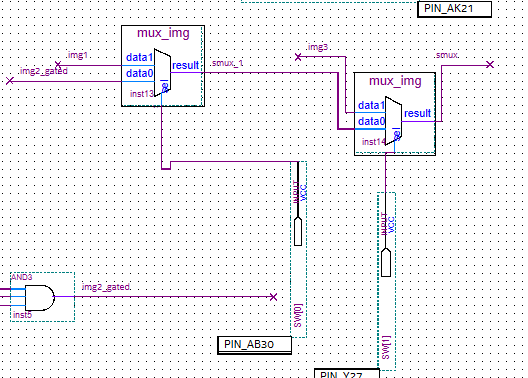
\includegraphics[width=0.90\textwidth]{muxes_to_filter_image_reusedfrompractice02.png}
		\caption{Diagrama BDF dos módulos \texttt{mux\_img} no \textit{top-level},
			responsáveis pela seleção da imagem exibida no VGA a partir das
			chaves \texttt{SW[0]} e \texttt{SW[1]}.}
		\label{fig:mux_bdf}
	\end{figure}
	
	% ============================================================
	%  SEÇÃO 4 — DISCUSSÃO DOS RESULTADOS
	% ============================================================
	\section{Discussão dos Resultados}
	
	\subsection{Comportamento do Filtro Sal e Pimenta via Rede \textit{Mesh}}
	
	Com a configuração diagonal ativa (n11 $\to$ n12 $\to$ n22 $\to$ n23) e
	\texttt{SW[0] = 0}, \texttt{SW[1] = 0}, o monitor VGA exibe a imagem filtrada
	resultante do processamento em cadeia pelos quatro nós da rede. A sequência
	de filtros MAX $\to$ MIN $\to$ MIN $\to$ MAX produz um efeito de suavização
	morfológica composta sobre a imagem binária, reduzindo pixels isolados de
	ruído impulsivo.
	
	As Figuras~\ref{fig:comb1}, \ref{fig:comb2} e \ref{fig:comb3} apresentam
	capturas do monitor VGA para as três configurações de roteamento disponíveis
	no \texttt{noc\_controller}. Em todos os casos, o resultado visual evidencia
	a remoção efetiva do ruído impulsivo, confirmando o funcionamento correto do
	roteamento XY e da lógica de seleção de modo em cada nó. A semelhança entre
	os três resultados demonstra que, independentemente da topologia do caminho
	ativo escolhida, a cadeia de quatro estágios morfológicos produz filtragem
	equivalente --- o que valida a consistência da implementação da NoC.
	
	\begin{figure}[H]
		\centering
		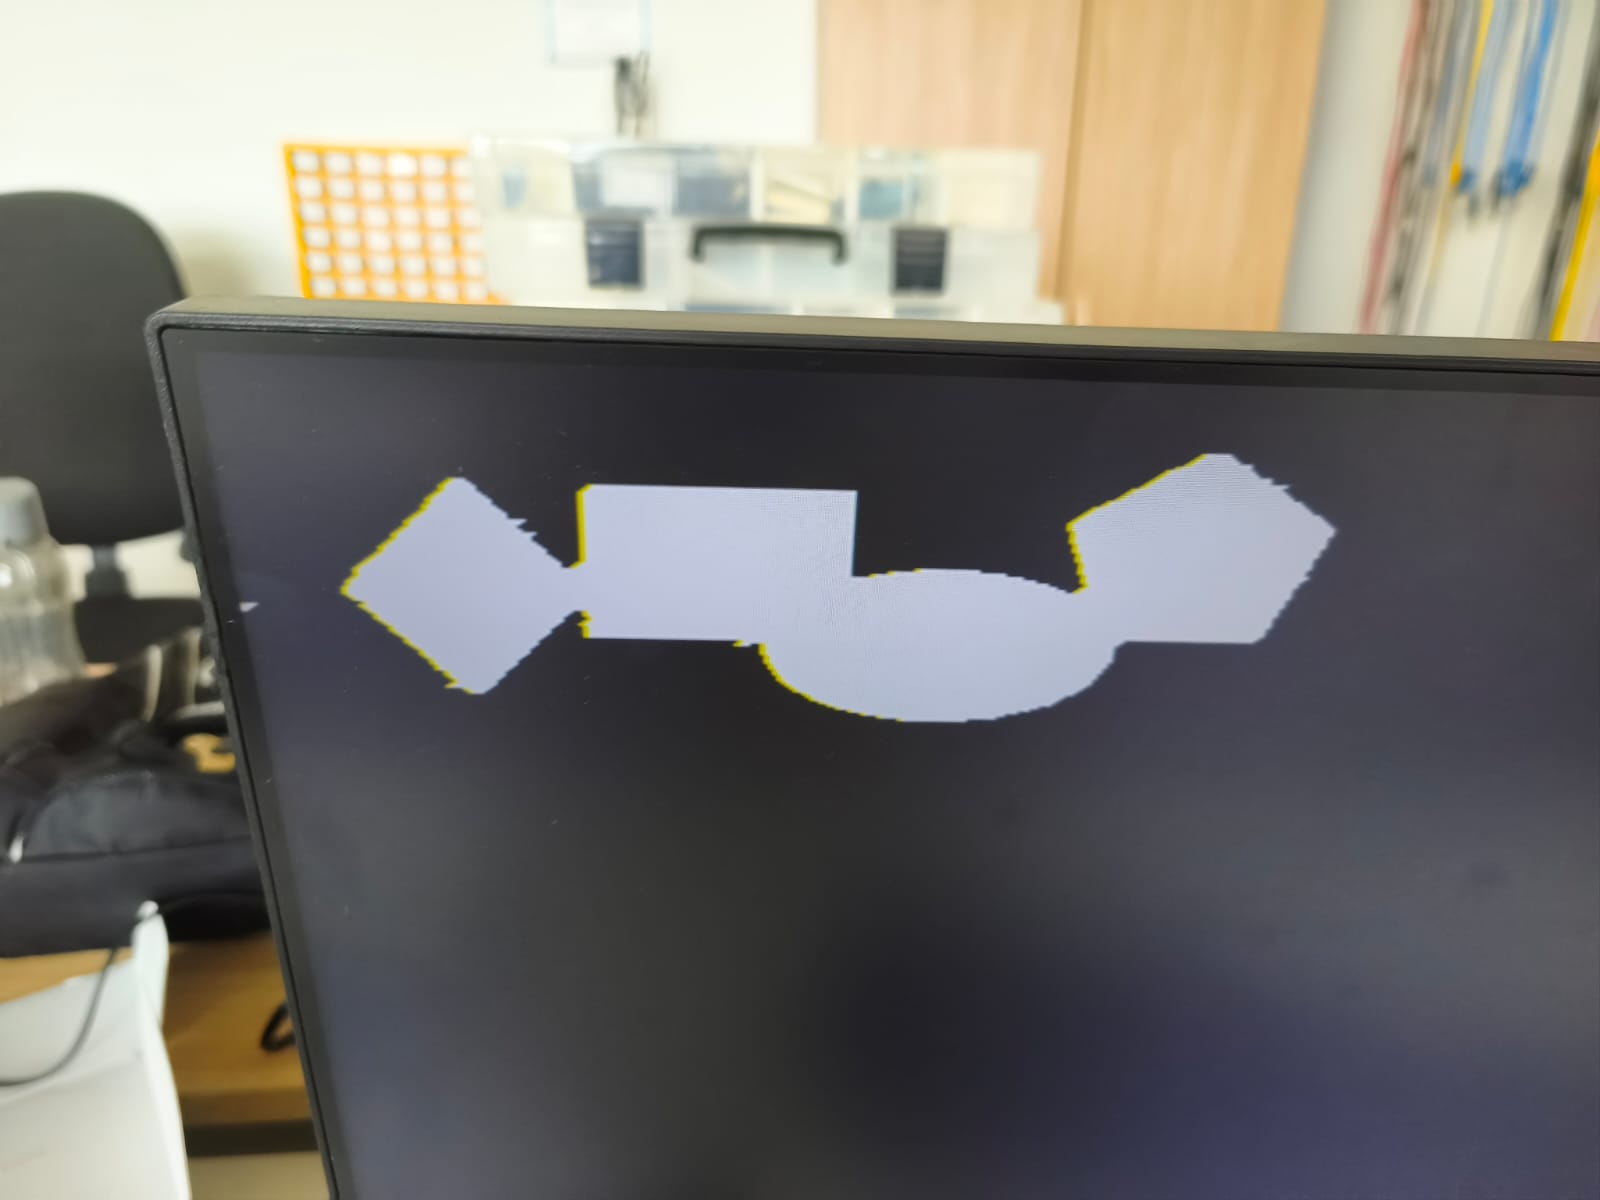
\includegraphics[width=0.75\textwidth]{filtered_image_combination1.jpeg}
		\caption{Imagem filtrada pela rede \textit{mesh} com configuração 1
			(coluna vertical: n10 $\to$ n11 $\to$ n12 $\to$ n13), exibida no
			monitor VGA com \texttt{SW[1:0] = 00}. O ruído impulsivo é removido
			com preservação das estruturas binárias originais.}
		\label{fig:comb1}
	\end{figure}
	
	\begin{figure}[H]
		\centering
		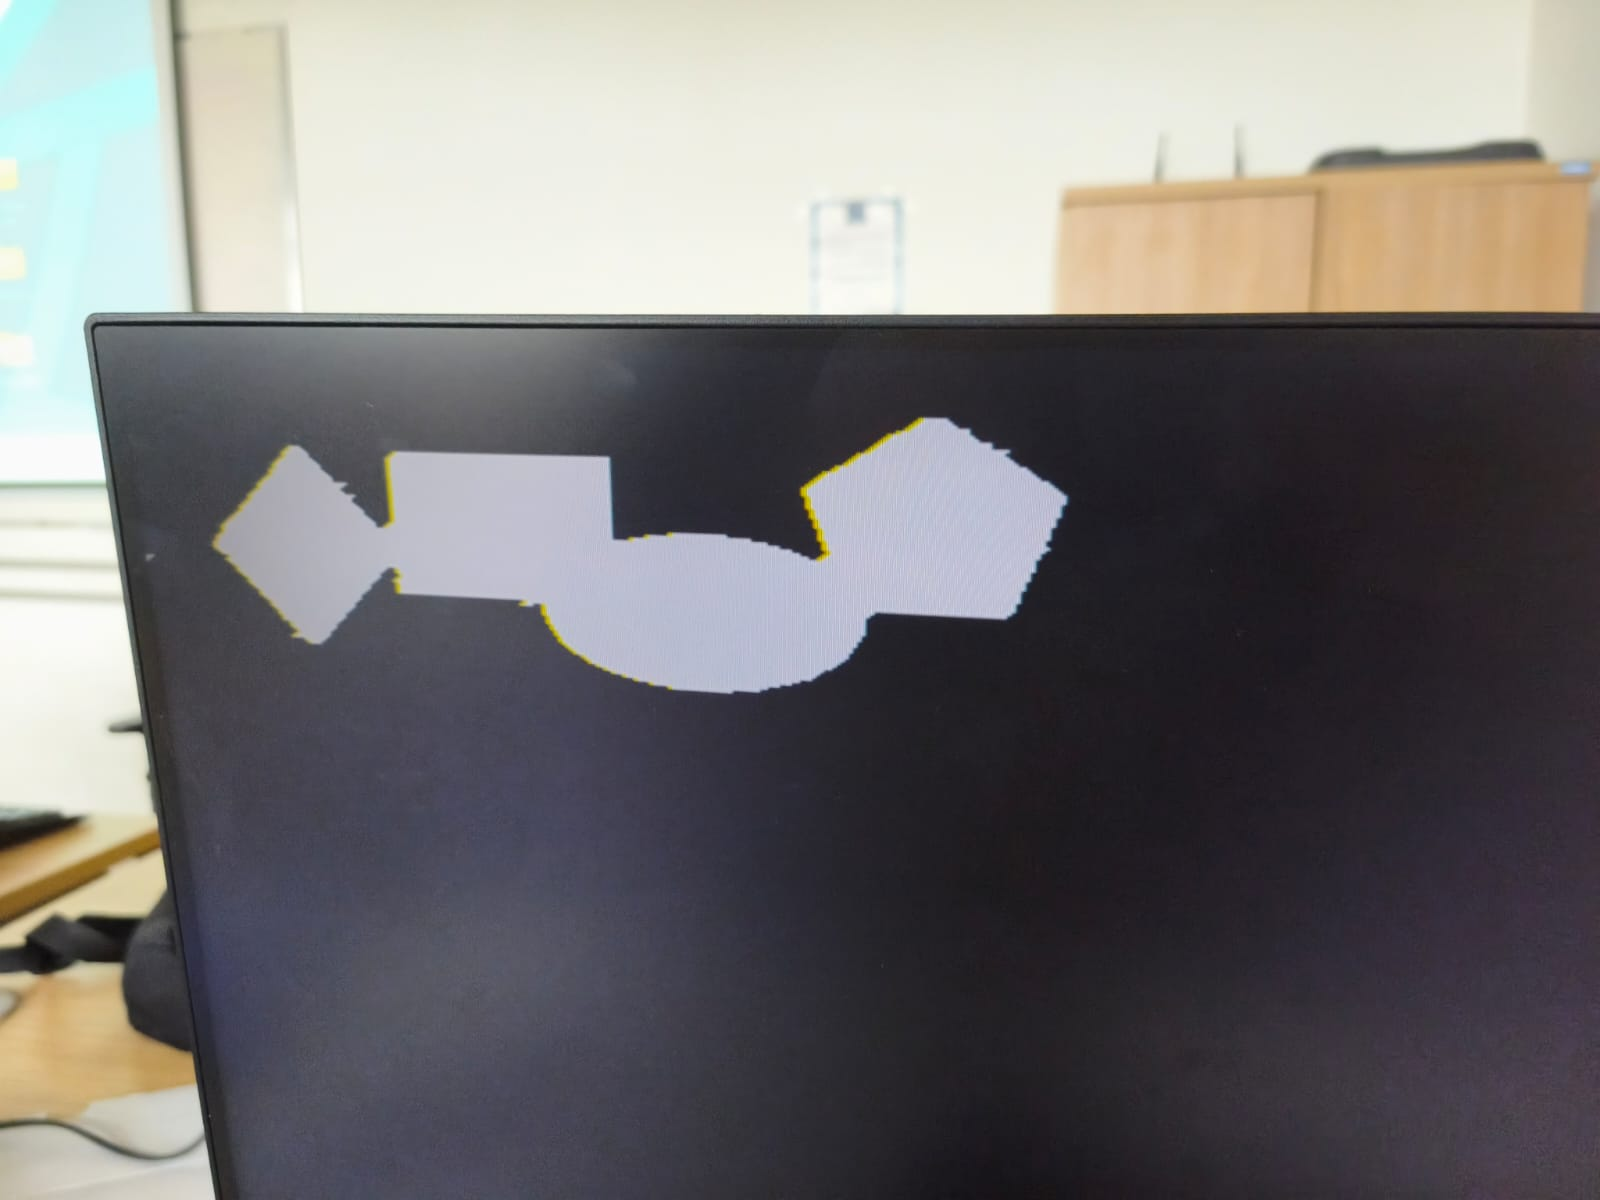
\includegraphics[width=0.75\textwidth]{filtered_image_combination2.jpeg}
		\caption{Imagem filtrada pela rede \textit{mesh} com configuração 2
			(grupo no topo em L: n00 $\to$ n01 $\to$ n11 $\to$ n12), exibida
			no monitor VGA com \texttt{SW[1:0] = 00}. O resultado é
			visualmente equivalente ao da configuração 1.}
		\label{fig:comb2}
	\end{figure}
	
	\begin{figure}[H]
		\centering
		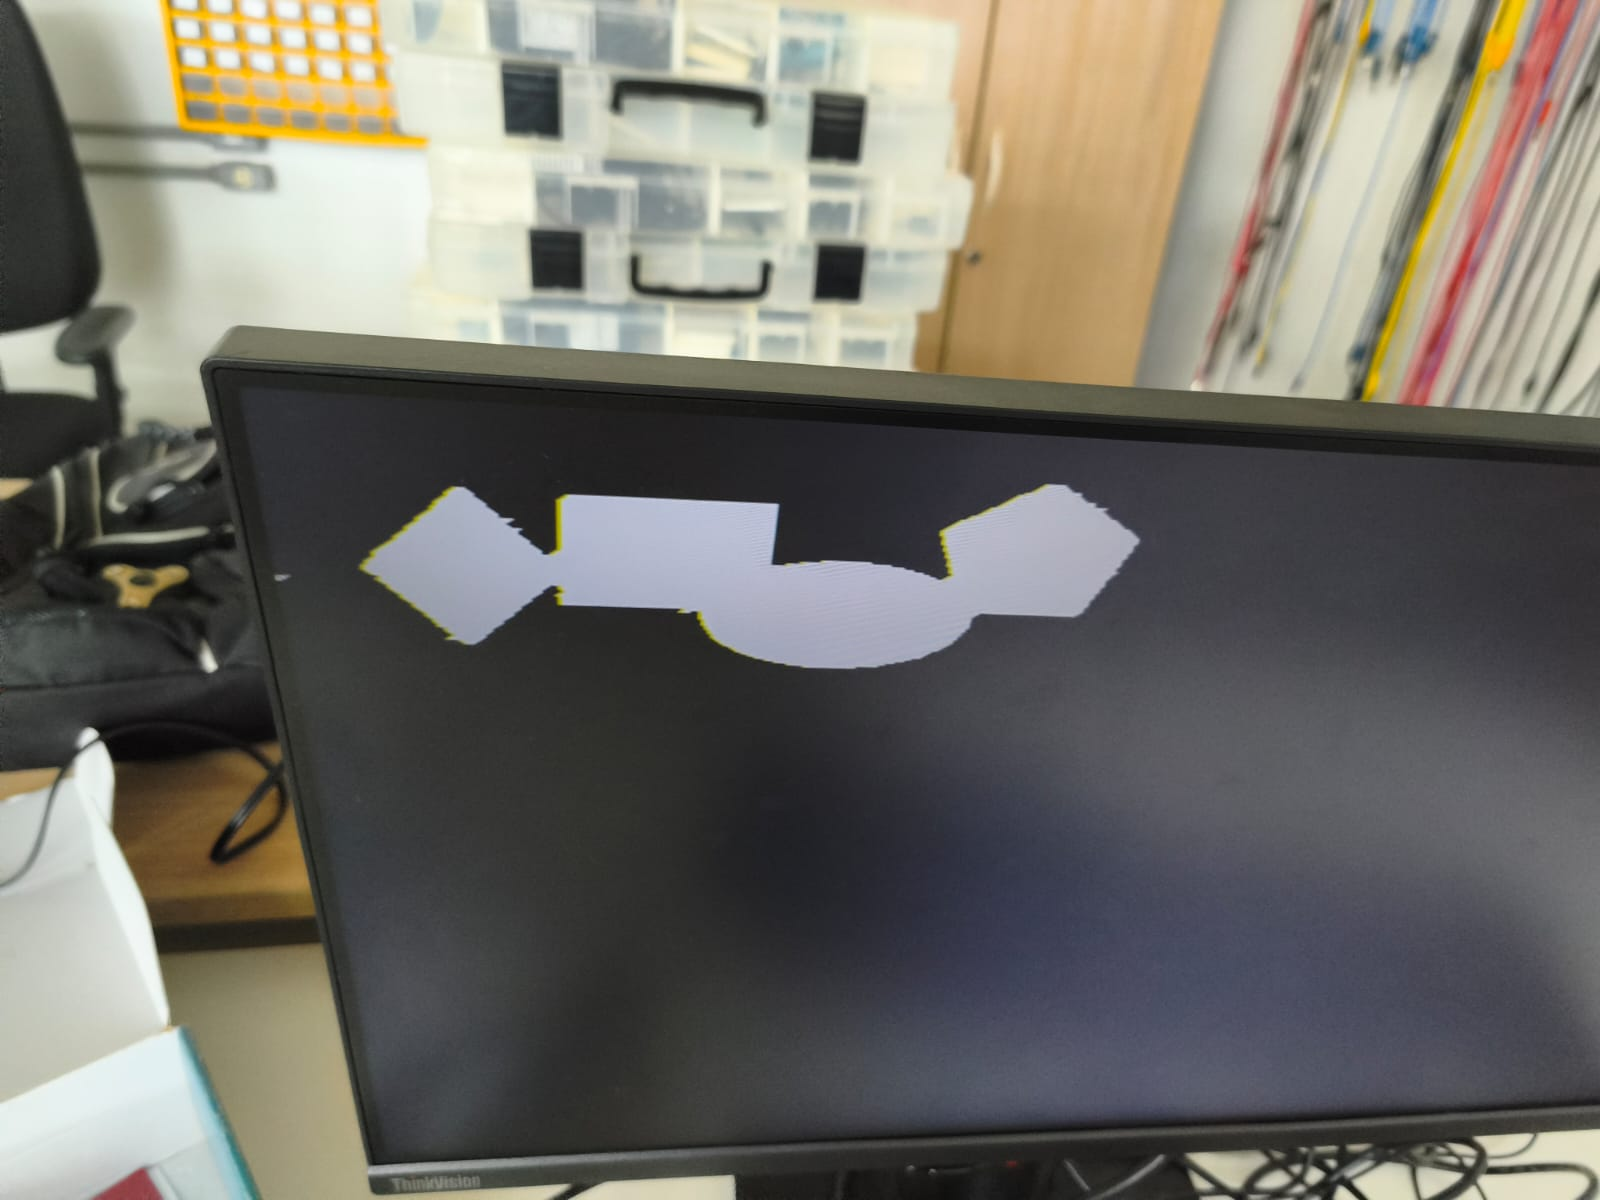
\includegraphics[width=0.75\textwidth]{filtered_image_combination3.jpeg}
		\caption{Imagem filtrada pela rede \textit{mesh} com configuração 3
			diagonal ativa (n11 $\to$ n12 $\to$ n22 $\to$ n23), exibida no
			monitor VGA com \texttt{SW[1:0] = 00}. A equivalência com as
			configurações anteriores confirma a corretude do roteamento XY
			para diferentes topologias de caminho.}
		\label{fig:comb3}
	\end{figure}
	
	\subsection{Flexibilidade de Configuração da NoC}
	
	A arquitetura proposta demonstra elevada flexibilidade: a simples alteração
	das constantes em \texttt{noc\_controller} permite explorar diferentes
	caminhos de processamento sem necessidade de modificação da fiação da
	\textit{mesh} ou dos nós individuais. As três configurações disponíveis
	(coluna vertical, grupo no topo e diagonal) produzem resultados visuais
	distintos, evidenciando como a topologia do caminho ativo influencia o
	comportamento do filtro composto.
	
	A configuração de coluna vertical (n10 $\to$ n11 $\to$ n12 $\to$ n13) aplica
	quatro estágios de filtragem em uma única coluna, maximizando a profundidade
	do processamento para aqueles pixels que percorrem o caminho. A configuração
	de grupo no topo explora nós em posições não alinhadas (formando um L),
	demonstrando que o roteamento XY é capaz de navegar caminhos com mudanças de
	direção. Em todos os casos, apenas os 4 nós do caminho realizam processamento
	efetivo; os demais 12 nós atuam exclusivamente como roteadores, transmitindo
	os dados sem modificá-los.
	
	\subsection{Clock Gating e Sincronismo com o VGA}
	
	O uso do clock gated (\texttt{clk2 = mask \& pclk \& on}) é fundamental para
	o correto funcionamento dos registradores de deslocamento internos ao
	\texttt{modulo\_sal\_e\_pimenta}. Como esses registradores constroem a janela
	deslizante de $3\times3$ pixels contando ciclos de clock, é imprescindível que
	o clock avance exatamente uma posição por pixel ativo da imagem. A inibição do
	clock fora da região ativa (\texttt{mask = 0}) e durante o \textit{blanking}
	VGA (\texttt{on = 0}) garante este comportamento.
	
	Contudo, o \textit{clock gating} combinacional implementado por portas AND
	pode introduzir \textit{glitches} no sinal de clock se os sinais de controle
	(\texttt{mask} e \texttt{on}) não forem estáveis durante as transições de
	subida do pixel clock. Em FPGA Cyclone II, recomenda-se o uso de primitivas
	dedicadas de \textit{clock gating} (como \texttt{ALTCLKCTRL}) para evitar
	este problema. Para as dimensões de imagem desta prática, os efeitos práticos
	são toleráveis e não comprometem a funcionalidade observada.
	
	\subsection{Latência do Caminho de Processamento}
	
	Cada nó do caminho de processamento introduz uma latência de 513 ciclos de
	clock ativos: 256 ciclos do primeiro registrador de deslocamento, mais 256
	ciclos do segundo, mais 1 ciclo do \texttt{shift\_3} (para completar a janela
	de 3 bits da linha corrente). Com 4 nós em série, a latência total é de
	$4 \times 513 = 2052$ ciclos de clock ativos. A uma taxa de 256 pixels por
	linha e 128 linhas, a imagem completa possui 32.768 pixels ativos por quadro,
	de forma que a latência de 2052 pixels corresponde a aproximadamente 8 linhas
	de imagem. Isto significa que os primeiros 8 valores de saída do filtro são
	inválidos (período de \textit{warmup}), o que pode ser observado como uma
	faixa escura nos primeiros pixels da imagem exibida.
	
	\subsection{Demonstração em Vídeo}
	
	O funcionamento completo do sistema --- incluindo a alternância entre as três
	configurações de roteamento da rede \textit{mesh}, a seleção entre imagem
	original, filtrada e com detecção de bordas via chaves da placa DE1, e a
	exibição em tempo real no monitor VGA --- foi registrado em vídeo e está
	disponível publicamente no YouTube:
	
	\begin{center}
		\url{https://www.youtube.com/shorts/twcA4ESBsww}
	\end{center}
	
	\noindent O vídeo demonstra a equivalência do resultado de filtragem entre as
	diferentes topologias de caminho configuradas no \texttt{noc\_controller},
	evidenciando a corretude do roteamento XY e a flexibilidade arquitetural da
	rede \textit{mesh} 4$\times$4.
	
	% ============================================================
	%  SEÇÃO 5 — CONCLUSÕES
	% ============================================================
	\section{Conclusões}
	
	Esta prática demonstrou com sucesso a implementação de uma rede
	\textit{mesh} 4$\times$4 para processamento digital de imagens em FPGA,
	com roteamento determinístico XY e cadeia de processamento configurável.
	As principais conclusões são:
	
	\begin{enumerate}
		\item \textbf{A topologia \textit{mesh} é naturalmente adequada para PDI
			em FPGA:} A regularidade da \textit{mesh} facilita tanto a implementação
		em hardware (fiação sistemática entre vizinhos) quanto a escalabilidade
		(a adição de linhas ou colunas segue o mesmo padrão de interligação). O
		uso de parâmetros estáticos por nó (\texttt{MY\_ADDR}) elimina lógica
		de endereçamento dinâmico, reduzindo o custo de área.
		
		\item \textbf{O roteamento XY garante ausência de \textit{deadlock} sem
			custo de tabelas de roteamento:} A decisão de roteamento em cada nó
		é puramente combinacional, baseada na comparação de 4 bits, e sintetiza-se
		em uma quantidade mínima de lógica. Não há estado de roteamento armazenado
		em nenhum nó, o que simplifica a verificação formal da correção do sistema.
		
		\item \textbf{O \texttt{noc\_controller} oferece reconfigurabilidade sem
			reprojeto da \textit{mesh}:} A separação entre a estrutura da rede
		(\texttt{mesh\_4x4}, \texttt{mesh\_node}) e o caminho de processamento
		(\texttt{noc\_controller}) permite alterar a topologia do filtro composto
		sem modificar a fiação da rede. Esta separação de preocupações é um
		princípio de projeto fundamental em arquiteturas NoC.
		
		\item \textbf{O clock gating é necessário mas requer cuidado em FPGA:}
		A inibição do clock da rede durante períodos de \textit{blanking} VGA
		é indispensável para o correto funcionamento dos registradores de
		deslocamento. O uso de portas AND combinacionais para \textit{clock gating}
		é funcional nesta escala, mas primitivas dedicadas seriam preferíveis em
		projetos maiores ou com requisitos de temporização mais estritos.
		
		\item \textbf{A latência acumulada de múltiplos estágios deve ser considerada:}
		O encadeamento de 4 módulos de filtro introduz uma latência de
		aproximadamente 8 linhas de imagem, visível nos primeiros pixels da
		saída filtrada. Em sistemas de processamento de vídeo em tempo real, esta
		latência deve ser contabilizada no projeto do pipeline de exibição.
	\end{enumerate}
	
	% ============================================================
	%  SEÇÃO 6 — REFERÊNCIAS BIBLIOGRÁFICAS (ABNT)
	% ============================================================
	\section{Referências Bibliográficas}
	
	\begin{thebibliography}{9}
		
		\bibitem{dally}
		DALLY, William J.; TOWLES, Brian.
		\textbf{Principles and Practices of Interconnection Networks}.
		San Francisco: Morgan Kaufmann, 2004.
		
		\bibitem{benini}
		BENINI, Luca; DE MICHELI, Giovanni.
		Networks on chips: a new SoC paradigm.
		\textit{IEEE Computer}, v. 35, n. 1, p. 70--78, jan. 2002.
		
		\bibitem{gonzalez}
		GONZALEZ, Rafael C.; WOODS, Richard E.
		\textbf{Processamento Digital de Imagens}.
		3. ed. São Paulo: Pearson Prentice Hall, 2010.
		
		\bibitem{embarcados1}
		EMBARCADOS.
		\textbf{Controlador VGA --- Parte 1}.
		Disponível em: \url{https://embarcados.com.br/controlador-vga-parte-1/}.
		Acesso em: 25 mai. 2026.
		
		\bibitem{embarcados2}
		EMBARCADOS.
		\textbf{Controlador VGA --- Parte 2}.
		Disponível em: \url{https://embarcados.com.br/controlador-vga-parte-2/}.
		Acesso em: 25 mai. 2026.
		
		\bibitem{quartus}
		INTEL CORPORATION.
		\textbf{Quartus Prime Standard Edition Handbook}.
		Disponível em: \url{https://www.intel.com/content/www/us/en/programmable/documentation/}.
		Acesso em: 25 mai. 2026.
		
		\bibitem{roteiro7}
		PEDRINO, Emerson Carlos.
		\textbf{Roteiro da Prática 7: Arquitetura Mesh para PDI}.
		São Carlos: UFSCar --- Departamento de Computação, 2026.
		Disponível em: $\langle$\url{https://ava.ufscar.br}$\rangle$. Acesso em: 25 mai. 2026.
		
		\bibitem{patterson}
		PATTERSON, David A.; HENNESSY, John L.
		\textbf{Organização e Projeto de Computadores: a Interface Hardware/Software}.
		5. ed. Rio de Janeiro: Elsevier, 2017.
		
		\bibitem{thomas}
		THOMAS, Donald E.; MOORBY, Philip R.
		\textbf{The Verilog Hardware Description Language}.
		5. ed. New York: Springer, 2002.
		
	\end{thebibliography}
	
	\end{document}